% ─── Slide: LoRA ablations ────────────────────────────────────────────────────
\begin{frame}{ADC-LoRA Ablations: Four Key Findings}
  \begin{columns}[T]
    \begin{column}{0.50\textwidth}
      \textbf{1. CE+KL consistently beats CE}
      \begin{itemize}
        \item \texttt{down+o, r4}: CE $\to$ 15.57; CE+KL $\to$ \better{14.33} ($-1.2$)
        \item \texttt{all 7, r4}: CE $\to$ 16.68; CE+KL $\to$ \better{14.03} ($-2.7$)
        \item FP teacher gives information CE alone cannot
      \end{itemize}
      \vspace{0.5em}
      \textbf{2. Rank saturates early}
      \begin{itemize}
        \item r=1: 15.90 \quad r=2: 15.60 \quad r=4: 15.57 \quad r=8: 15.24
        \item Most capacity captured at r=1; higher ranks: diminishing returns
      \end{itemize}
      \vspace{0.5em}
      \textbf{3. First 8 layers beat last 8}
      \begin{itemize}
        \item \texttt{first8}: 16.64 \qquad \texttt{last8}: 20.08
        \item Early layers accumulate and \emph{propagate} ADC errors downstream
      \end{itemize}
      \vspace{0.5em}
      \textbf{4. Seeds stable} ($\sigma \approx 0.07$ across seeds 1/2/3)\\
      End-to-end pipeline (PTQ + LoRA) is reproducible.
    \end{column}
    \begin{column}{0.46\textwidth}
      % 4 mini panels
      \iffalse
        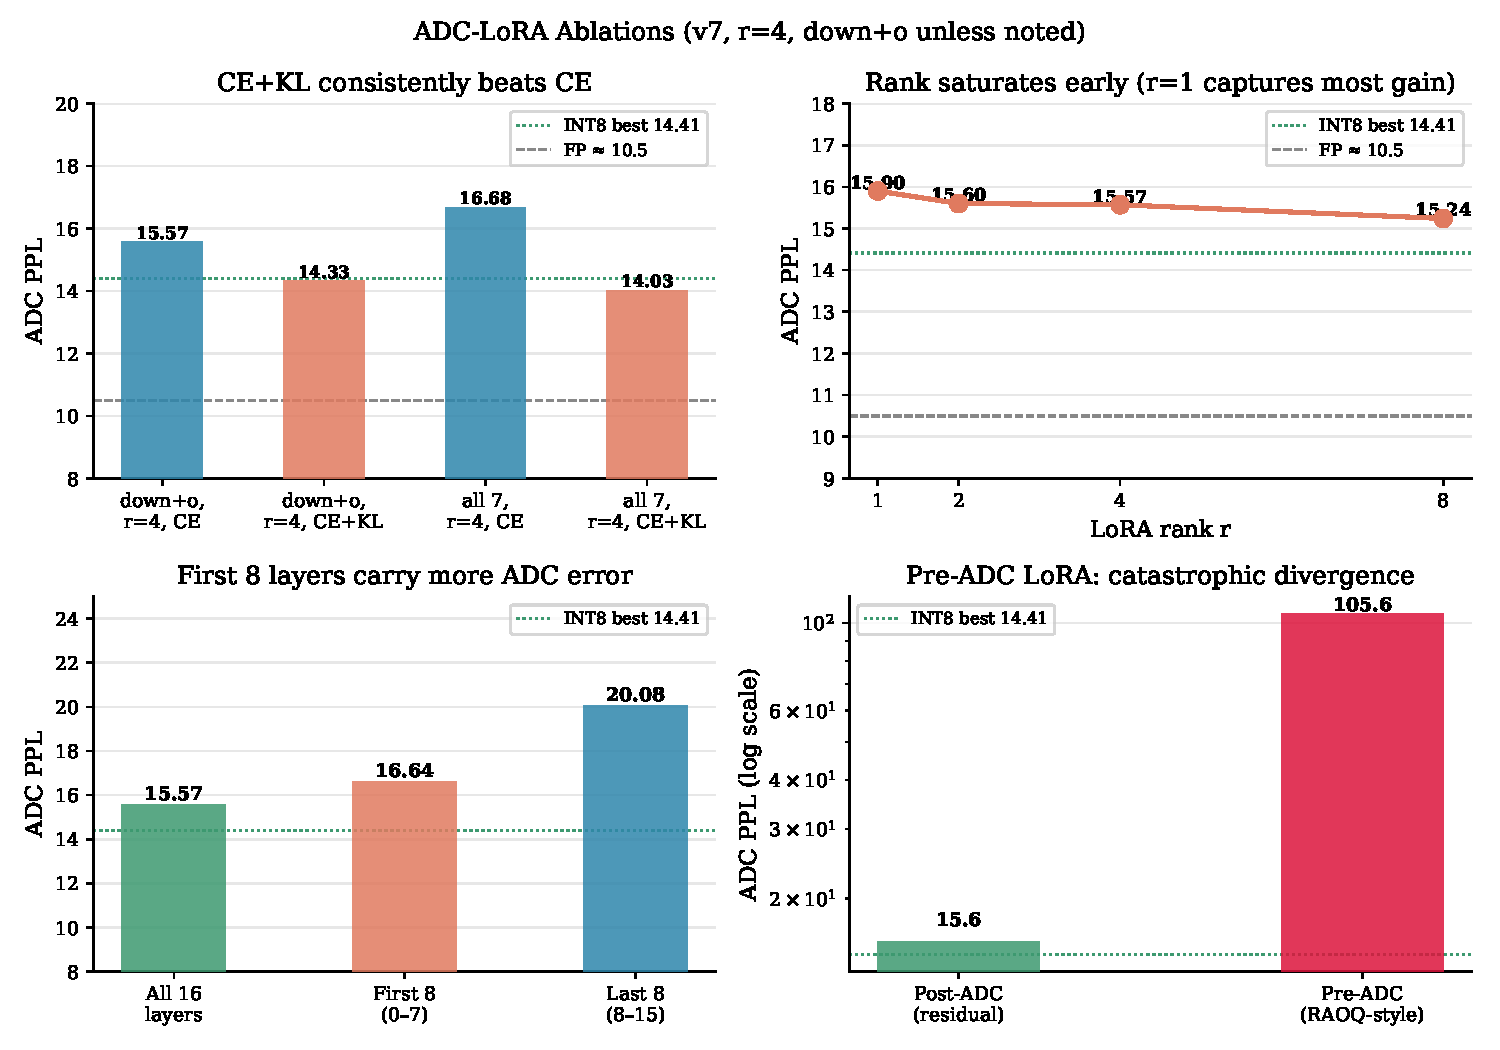
\includegraphics[width=\linewidth]{figs/plot_lora_ablations_grid.pdf}
      \else
        \figplaceholder[0.82\textheight]{2$\times$2 grid of small bar charts.
          Top-left: CE vs CE+KL (down+o and all7).
          Top-right: rank sweep r=1/2/4/8 (down+o, CE+KL).
          Bottom-left: first8 vs last8 vs all16 (ADC PPL).
          Bottom-right: post-ADC vs pre-ADC LoRA — show catastrophic pre-ADC result.}
      \fi
    \end{column}
  \end{columns}
\end{frame}
